\documentclass[a4paper]{article}

\usepackage{array}
\usepackage{placeins}
\usepackage{listings}
\usepackage{hyperref}
\usepackage{enumitem}

\usepackage{hopsantut}

\begin{document}
\maketitle{Exporting Models to Simulink}

\section*{Introduction}
The Matlab and Simulink tools are widely used for modeling and simulation, especially the fields of control and system engineering. 
This tutorial will show how Hopsan models can be exported to Simulink.
This enables powerful development methods, such as testing a controller made in Simulink on a model built in Hopsan.
It can also be used for connecting Hopsan with other programs through Simulink, or to run real-time simulations.
Furthermore, Simulink has powerful toolboxes, such as system identification, otimization and control, which can be used on Hopsan models.

\section*{Requirements}
To do this tutorial, you will need Matlab/Simulink (of a relatively new version).
You also need a compatible C++ compiler, usually Microsoft Visual C++ (MSVC).
The version of MSVC depends on the version of Matlab.
See \url{http://www.mathworks.com/support/compilers} for more information.
It is advised 

%Kanske ska skriva en lista med de senaste Matlab-versionerna och deras compilers här?

\section*{Exporting a Model to Simulink}
We will now export a model of a position servo from Hopsan to Simulink.
Then we will build a simple controller in Simulink, and connect it to the exported model.
It will also be demonstrated how you can change the model in Hopsan without having to redo the export process.

\begin{enumerate}
\tutitem{Open the model}
Open the \textit{Position Servo} example model. It can be found on the welcome screen, or through the \textit{Help} menu. When opened, it will look like this:
 
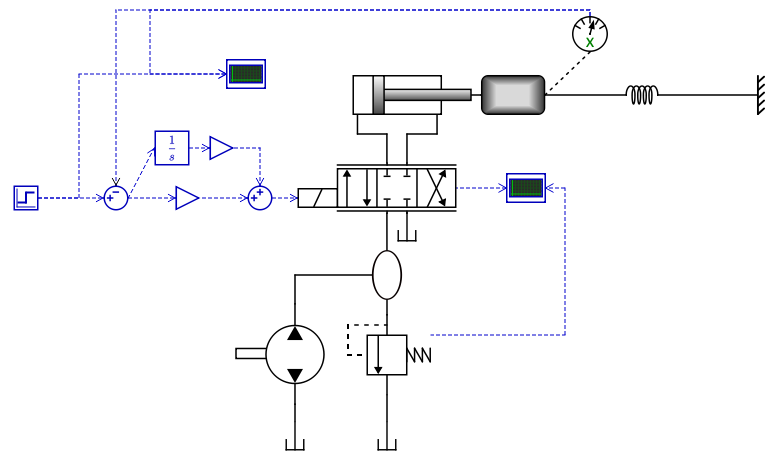
\includegraphics[height=8cm]{gfx/simulink/model1.png}

\textit{Remove the controller in Hopsan}
The model in Hopsan contains a PI-controller. 
We will not need this, since we are going to build a controller in Simulink instead.  
Remove the controller, so that the model looks like below:

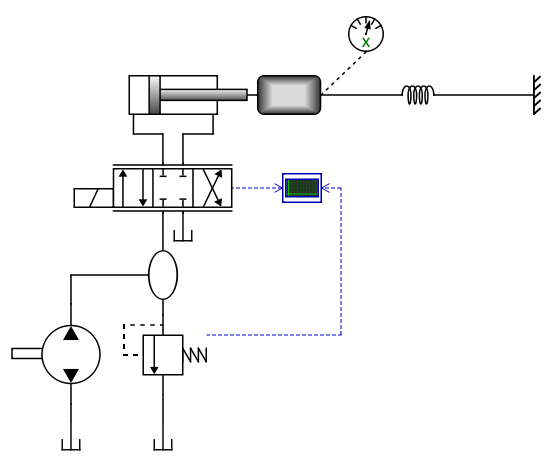
\includegraphics[height=8cm]{gfx/simulink/model2.png}

To communicate between Simulink and Hopsan we need some interface ports.
These are defined by \textit{Interface} components in Hopsan.
We want to use control signal to the valve for input, and the actual position of the piston for output.
Add one input and one output component:

\vspace{5pt}
\foldericon{0}{Connectivity}
\component{1}{Input Interface Component}
\component{1}{Output Interface Component}
\vspace{5pt}

Connect the input component to the directional valve and name it "u".
Then connect the output component to the position sensor and name it "y".
The model should then look like this:

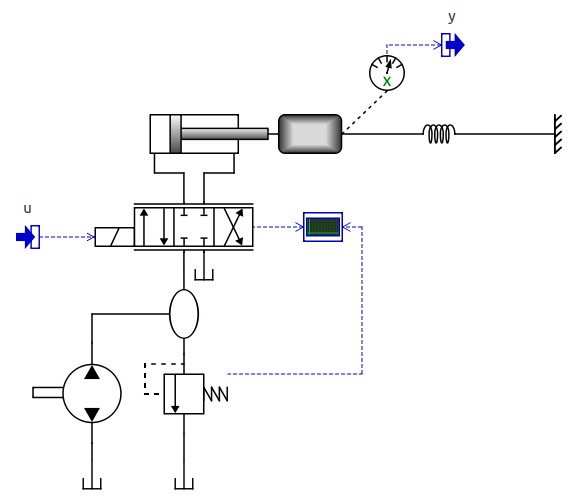
\includegraphics[height=8.73753cm]{gfx/simulink/model3.png}

\tutitem{Export the model}
Now create a new empty folder anywhere on your hard drive. Then click the export to S-function button in the toolbar:

\icon{0}{gfx/Hopsan-ExportSimulink.png}{Export model to Simulink S-function}

The program will ask you whether or not you want to disable port labels.
This is not necessary for most reasonably new versions of Matlab. 
Click OK, then browse to the folder you created and select it. 
Hopsan will then export all required files to there.

\tutitem{Configure Matlab}
Now start Matlab and wait for it to open. 
It is necessary to configure Matlab so that it uses the correct compiler. 
This is done with the \texttt{mex -setup} command. 
Run it, choose Microsoft Visual Studio, then select yes (y). 
It should look like below. 

%Ställ in rätt kompilator
\lstset{
    breaklines     = true,
    basicstyle	   = \footnotesize\ttfamily
}
\begin{lstlisting}
>> mex -setup
 
Welcome to mex -setup.  This utility will help you set up  
a default compiler.  For a list of supported compilers, see  
http://www.mathworks.com/support/compilers/R2013b/win64.html 
 
Please choose your compiler for building MEX-files: 
 
Would you like mex to locate installed compilers [y]/n? y
 
Select a compiler: 
[1] Microsoft Software Development Kit (SDK) 7.1 in C:\Program Files (x86)\Microsoft Visual Studio 10.0 
 
[0] None 
 
Compiler: 1
 
Please verify your choices: 
 
Compiler: Microsoft Software Development Kit (SDK) 7.1 
Location: C:\Program Files (x86)\Microsoft Visual Studio 10.0 
 
Are these correct [y]/n? y
\end{lstlisting}

If the Visual Studio compiler does not appear, it is not installed correctly, or the installed version is not compatible with your version of Matlab. 
Consult the Matlab user manual for more information.

\tutitem{Compile the S-function}
Set Matlab's working directory to the folder you exported the model to.
One of the exported files from Hopsan is a compilation script, called \texttt{HopsanSimulinkCompile.m}.
Running this script will compile the S-function from the exported source code using the compiler selected above. 
Call the script by writing the file name in the console. 
If successful, it should look like this: 

\begin{lstlisting}
>> HopsanSimulinkCompile
Compiling S-function from Hopsan model...
Finished.
\end{lstlisting}

If you look in the folder, you can see that a new file called \texttt{Position\_Servo.mexw64} (or \texttt{Position\_Servo.mexw32} for 32-bit systems) was created. This is the compiled S-function, which we can now use in Simulink.

\tutitem{Start Simulink}
Start Simulink by clicking on the icon or by writing \texttt{simulink} in the console. Then create a new empty model.

\tutitem{Open the Hopsan model in Simulink}
Now locate the Simulink block called "S-function", located under "\textit{Simulink\textbackslash User-Defined Functions}". 
Drag it to your model to add it. 
Then double-click on it and change the parameter "S-function name" to the file name of the S-function without file extension, i.e. "Position\_Servo". 
Then click ok to close the dialog.
The block should now look like this:

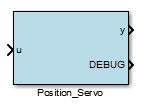
\includegraphics{gfx/simulink/sfunction.png}

We have one input called "u" ad one output called "y", representing the input and output interface components in Hopsan.
There is also an output called "DEBUG".
This is used to tell us if something is wrong.
It should normally be zero.

\tutitem{Build a simple controller in Simulink}
Simulink is commonly used by control engineers to construct control algorithms. 
We will now build a very simple proportional controller, to demonstrate how this can be used on a Hopsan model.
Add a Step block as a reference signal, a Subtract and a Gain block for the controller and a Scope to view the results.
Connect them as the picture below:

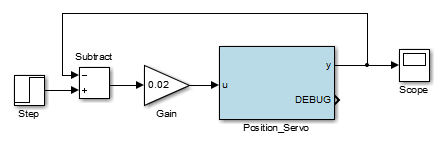
\includegraphics{gfx/simulink/simulinkfeedback.png}

Change the "Final value" parameter of the step to 0.5 and the "Gain" parameter in the gain block to 0.02. Set the simulation stop time to 2 seconds.

\tutitem{Simulate the model in Simulink}
Now press the \textit{Run} button in Simulink. After the simulation as finished, double-click on the scope. It may be necessary to uncheck the \textit{Limit number of data points} option to get see all results. If everything works correctly, the result should look like this:

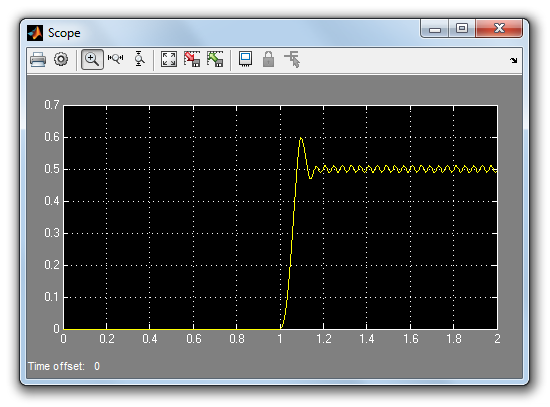
\includegraphics[width=0.6\linewidth]{gfx/simulink/simulinkplot.png}

If you like to, you can verify the results by creating a similar controller in Hopsan and run the same simulation there.

\tutitem{Modify the Hopsan model}
As long as the interface components are not changed, it is possible to modify the Hopsan model without re-compiling.
Try changing the mass component in Hopsan to a mass with friction:

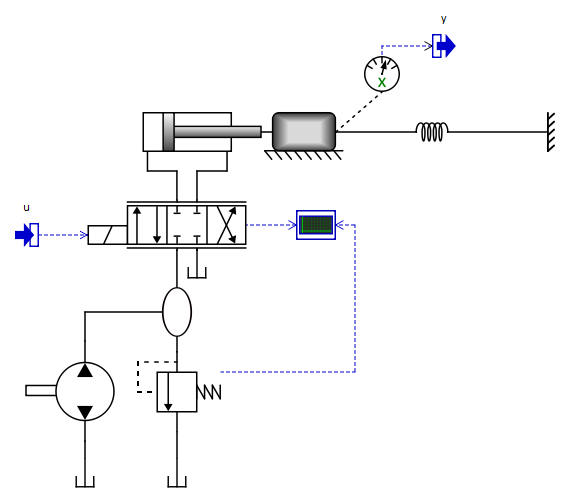
\includegraphics[height=8.73753cm]{gfx/simulink/modifiedmodel.png}

Also change the damping parameter (B\_p) in the piston component to 1000.
Then click \textit{save as} (not \textit{save}!) and overwrite the model \textit{in the exported directory}.
This is the model used by Simulink.
Then simulate from Simulink again and look at the results.
The results are now different, even though we did not re-export the model.

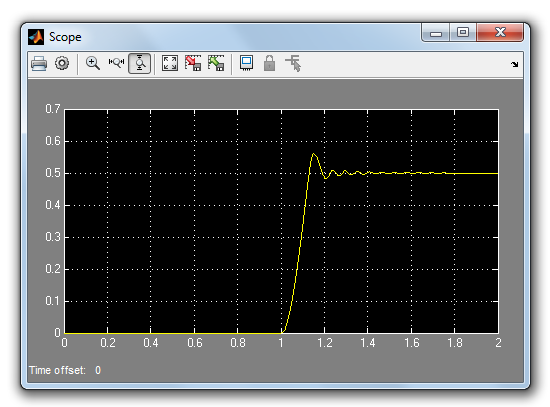
\includegraphics[width=0.6\linewidth]{gfx/simulink/simulinkplot2.png}

It is thus possible to modify the model from Hopsan without exporting it again, as long as interface components are not changed or renamed.

\end{enumerate}

\end{document}